\documentclass{beamer}
\usepackage[utf8]{inputenc}
\usepackage[T1]{fontenc}
\usepackage{lmodern}
\usepackage[english]{babel}
\usepackage{lsfolien}
\usepackage{hyperref}

\myfootline{System Modelling and Semantic Web -- Summer Term 2022}{Victor Jüttner}

\title{Hands on Systematic Innovation\\
	Problem Solving Tools - Measurement Problems
	\vskip1em}

\subtitle{Presentation in the Module 10-202-2312}

\author{Victor Jüttner}

\date{24. May 2022}


\begin{document}

	\begin{frame}[plain]
		\maketitle
	\end{frame}

	\section{Motivation}
	
	\begin{frame}{Measuring for Mechanics}
		\begin{columns}
			\column{.4\textwidth}
			\begin{itemize}
				\item Dimensions needed for functionality
				\item Need to confim all given dimensions
				\item Know exactly how to measure them
				\item No unnecessary measuring
			\end{itemize}
			\column{.6\textwidth}
			\begin{figure}
				\centering
				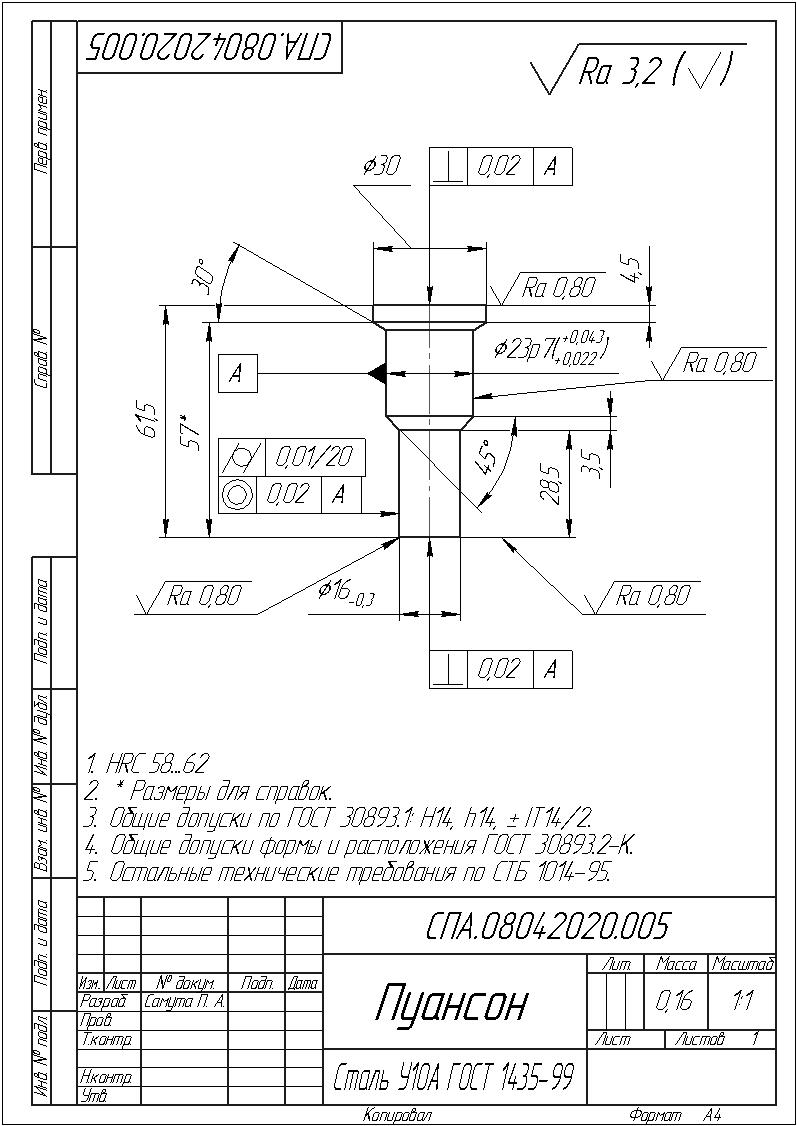
\includegraphics[width=.7\textwidth]{img/Technical_drawing_CAD.jpg}
				\caption{Technical drawing \href{https://commons.wikimedia.org/w/index.php?curid=113182825}{by Pavelsamuta1}}
			\end{figure}	
		\end{columns}
	\end{frame}

	\begin{frame}{Measuring Code Quality}
		\begin{itemize}
			\item Why?
				\begin{itemize}
					\item Readability
					\item Maintainability
					\item Reusability
				\end{itemize}
			\item What?
				\begin{itemize}
					\item Complexity
					\item Number of defects
					\item Standards
				\end{itemize}
			\item How?
				\begin{itemize}
					\item Count lines of code
					\item Cyclomatic Complexity
					\item Defect Density
					\item Count comment lines
				\end{itemize}
		\end{itemize}
	\end{frame}

	\begin{frame}{Measurement in Business Context}
		\begin{itemize}
			\item Financial success
			\item Customer satisfaction
			\item Production costs
			\item Brand value
			\item Product Quality
		\end{itemize}
	\end{frame}

	\begin{frame}{Measuring}
		\begin{itemize}
			\item What to Measure and Why to Measure It?
			\item How to Measure?
			\item Case Studies
		\end{itemize}
	\end{frame}


	\section{What To Measure and Why To Measure It?}
	
	\begin{frame}{Measuring popular amongst Manager}
		\begin{itemize}
			\item 'you don’t fatten a cow by weighing it'
			\item 'what gets measured gets done'
			\item 'the most important numbers are unknown and unknowable'
		\end{itemize}
	\end{frame}
	
	\begin{frame}{Ideality Equation}
		Used throughout the systematic innovation methodology. \\ Here for the individual elements or the whole system.
		\begin{equation*}
			\text{Ideality} = \text{Perceived} \left(\frac{\text{Benefits}}{\text{Cost} + \text{Harm}}\right)
		\end{equation*}
		\begin{description}
			\item[Costs] Most popular element and easy to measure.
			\item[Harm] Waste, environmental- and sustainability issues.
			\item[Benefits] Value of product/service from perspective of receiver.
			\item[Perceived] Respects complexity and uncertainty of intangibles.
		\end{description}
	\end{frame}

	\begin{frame}{Need for overall Ideality}
		\begin{figure}
			\centering
			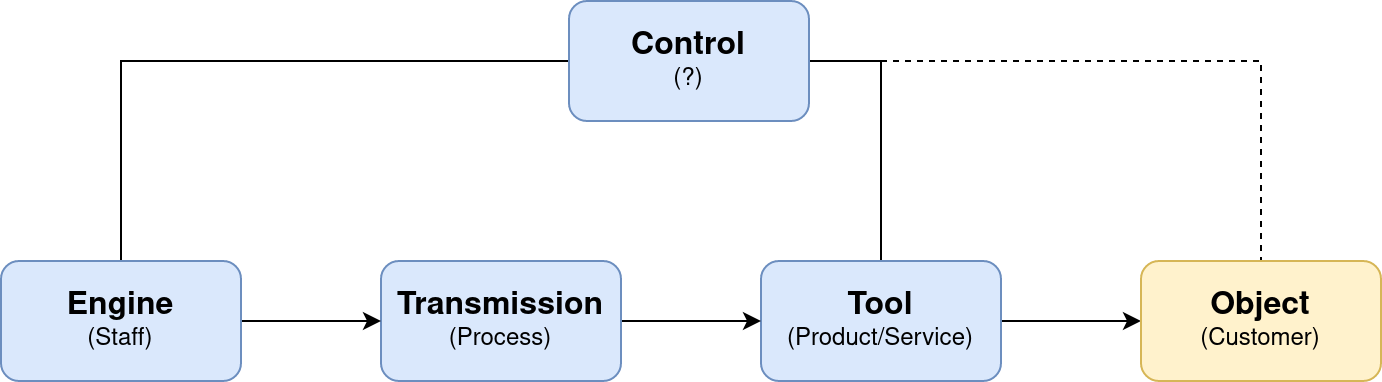
\includegraphics[width=\textwidth]{img/control3.png}
			\caption{Feedback and Control in a viable System (adapted from D. Mann "Hands on Systematic Innovation for Business and Management", p. 354)}
		\end{figure}
	\end{frame}

	\begin{frame}{Complexity}
		\begin{figure}
			\centering
			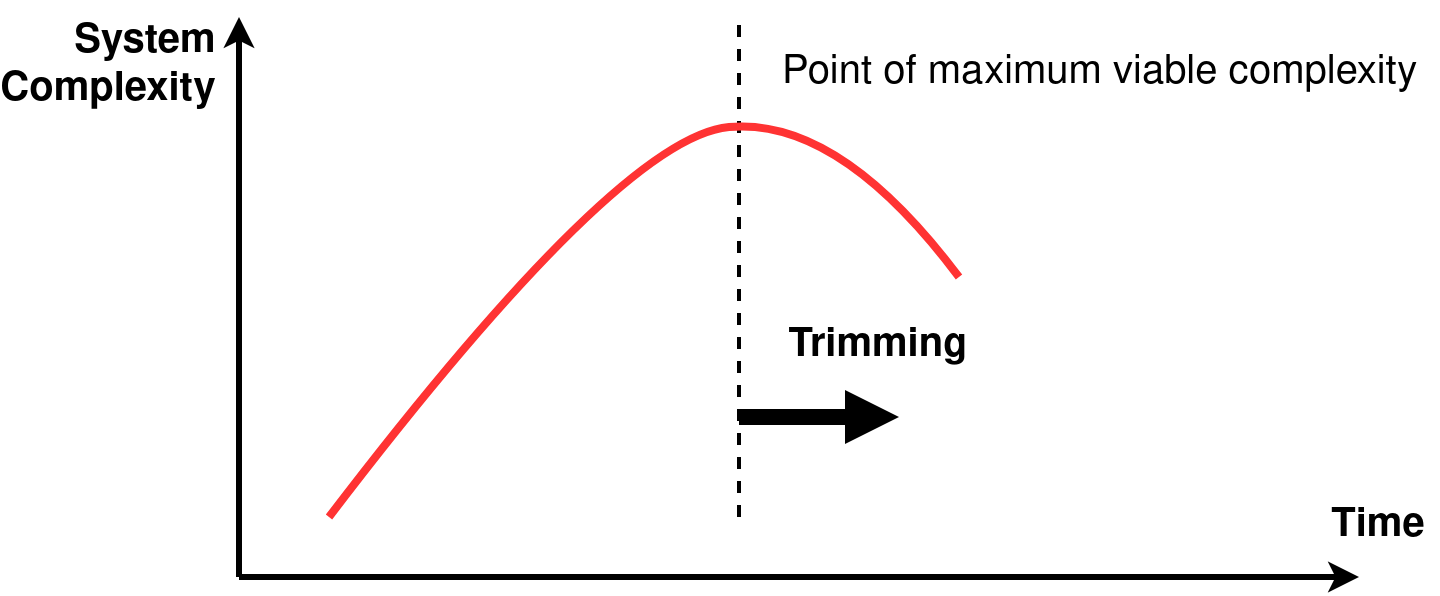
\includegraphics[width=\textwidth]{img/complexity2.png}
			\caption{Complexity Trend (adapted from D. Mann "Hands on Systematic Innovation for Business and Management", p. 355)}
		\end{figure}
	\end{frame}

	\begin{frame}{Seminarconcept - Triz Methodology}
		\begin{itemize}
			\item to sharpen intended effects in functional modelling as an Ideal Final
			Result or Ideal Machine,
			\item to identify negative (harmful) effects occurring during implementation, 
			\item to localise such problems as contradictory behaviour in a delimitable
			"operational zone", 
			\item and finally to resolve such contradictions by transforming a "system as
			it is" into a "system as required".
		\end{itemize}
	\end{frame}
	
	\section{How to measure}
	

	\begin{frame}{(A) Modify the system so that there is no need to make the detection or measurement}
		\begin{itemize}
			\item Eliminate the need for measurement
			\item Use already existing resources
			\item Increase company transparency
			\item Integrate measures into one another
			\item Be careful!
		\end{itemize}
	\end{frame}

	\begin{frame}{(B) Make the detection or measurement on a copy, image or replica of the object or system}
		\begin{itemize}
			\item Beta test networks as seperate microcosm
			\item Test audiences
			\item Customer feedback through internet-based forms
			\item Virtual customers?
		\end{itemize}
	\end{frame}

	\begin{frame}{(C) Transform the problem into one involving successive measurement of changes}
		\begin{itemize}
			\item Measure delta's between successive measurements
			\item Key/Mouse-click rate to detect competence of user
			\item Response times in a car to measure intoxication
			\item Predict frequency of future measurements
			\item Identify proximity to potential non-linearities by changing frequency
		\end{itemize}
	\end{frame}

	\begin{frame}{(D) Add a new element (communication or person or element) to provide an easily detectable parameter related to the parameter required to be measured or detected}
		\begin{itemize}
			\item Mystery Shopper, e.g. on customer service
			\item Suggestions schemes
			\item Notice boards
			\item Cookies
			\item Interactive TV
			\item GPS tracking system
		\end{itemize}
	\end{frame}

	\begin{frame}{(E) If it is not possible to modify the system, then introduce an easily detected element to the surrounding environment}
		\begin{itemize}
			\item Bring in a temporary consultant
			\item CCTV cameras
			\item Heisenberg Uncertainty Principles
		\end{itemize}
	\end{frame}

	\begin{frame}{(F) If it is not possible to introduce an easily detectable element into the environment surrounding a system, obtain the desired measurement by detecting changes in something already in the environment}
		\begin{itemize}
			\item Use friends and family to obtain information on morale
			\item Use press to measure changes in customer market suggestion
			\item Key-presses on a computer keyboard
			\item Audience noise levels
		\end{itemize}
	\end{frame}

	\begin{frame}{(G) Make use of psychological effects to help make the measurement}
		\begin{itemize}
			\item Telling someone they can't have something is a good way of making them want it: Feedback mechanism
			\item Most people have the desire to be helpful
			\item People need certain amount of stimulus before they commit
			\item Be inclusive when formulating questions
			\item Bad news travels faster than good news
			\item The more you tell people the more they think you're hiding
		\end{itemize}
	\end{frame}

	\begin{frame}{(H) Use emotional effects to help to make the measurement}
		\begin{itemize}
			\item Identification and use of exciters
			\item Identification and use of customer hot buttons
			\item Emphatic listening
		\end{itemize}
	\end{frame}

	\begin{frame}{(I) Use the inverse or opposite system to make the measurement}
		\begin{itemize}
			\item Measure empty space, things that aren't present
			\item Measure non-customers
		\end{itemize}
	\end{frame}

	
	\section{Case Studies - Who? When? Where}
	
	\begin{frame}{Measuring Business Performance}
		\begin{block}{What to measure?}
			Business often measure success based on what is measurable rather than what is important.
		\end{block}
		
		\begin{itemize}
			\item Photographic paper industry
			\item Regular measurements: streams of incoming and outgoing resources
			\item What is the main useful function?
			\item Use knowledge about how customers use product to improve, and know what to measure
		\end{itemize}

	\end{frame}

	\begin{frame}{Project Management System Measurements}
		\begin{block}{Relationship measurement and resources}
			The ideal final result project management measurement requires no additional resource to acquire it.
		\end{block}
		
		
		\begin{itemize}
			\item Global statistics show that 85\% of project end late, over-budget or under-specification
			\item Common-sense approach: If there isn't enough data to be successful, hire more project managers
			\item Measurement should become self-sustaining without further resources
		\end{itemize}
	\end{frame}


	\begin{frame}{Measuring best practice}
		\begin{itemize}
			\item Measurement methods most needed when system is in evolutionary development and is suffering from inadequate feedback and control mechanisms.
			\item When a new function is added to the system
			\item Define in simple functional terms the measurement required from the system under consideration.
			\item Is the measurement actually required by thinking about the useful
			function it is intended to deliver?
		\end{itemize}
	\end{frame}
	
	
	

\end{document}